\begin{activity}{Plate Cooling and Fourier Series}

\section*{Purpose}
To understand how imposing a fixed lithospheric thickness modifies transient
cooling and why Fourier series naturally arise in plate cooling models.

{\color{red}
\section*{Learning Outcomes}

By the end of this activity, you should be able to:
\begin{itemize}
  \item Explain the physical meaning of each Fourier mode in the plate cooling solution and relate mode index $n$ to thermal wavelength.
  \item Describe why short-wavelength (high-$n$) modes decay faster than long-wavelength modes.
  \item Compare plate cooling and half-space cooling predictions for bathymetry and heat flow, and identify when they diverge.
  \item Connect the Fourier mode concept to the spectral filtering ideas from gravity and magnetics (Weeks 6--7).
\end{itemize}
}

\section*{Concept}
Plate models introduce a basal boundary condition at a fixed depth, representing
the lithosphere--asthenosphere boundary.

\section*{Mathematical Form}
The temperature field can be expressed as a Fourier series:
\[
T(z,t) = \sum_{n=1}^{\infty} A_n
\sin\!\left(\frac{n\pi z}{L}\right)
\exp\!\left(-\frac{n^2 \pi^2 \kappa t}{L^2}\right).
\]

\section*{Tasks}
\begin{enumerate}
  \item Explain how the index $n$ relates to thermal wavelength.
  \answerbox[2cm]
  \item Why do short-wavelength modes decay faster than long-wavelength modes?
  \answerbox[3cm]
  \item Compare thermal evolution predicted by plate cooling and half-space cooling.
  \answerbox[3cm]
\end{enumerate}

\section*{Geological Interpretation}
\begin{itemize}
  \item Plate thickness limits lithospheric growth.
  \item Explains flattening of bathymetry and heat flow for old oceanic plates.
\end{itemize}

\section*{Connection}
Relate Fourier modes to spectral filtering concepts used previously in gravity
and magnetic field analysis.

\answerbox[3cm]

{\color{red}
\section*{Key Ideas}

\textbf{A fixed plate thickness imposes a lower boundary condition.} By setting the temperature at the base of the lithosphere to the mantle potential temperature, the plate model prevents unbounded cooling. The lithosphere approaches a steady-state thickness rather than growing indefinitely.

{\color{blue}
\textbf{Each Fourier mode has its own decay timescale.} The exponential factor $\exp(-n^2\pi^2\kappa t/L^2)$ shows that high-order modes (short wavelengths) decay much faster than low-order modes (long wavelengths). After sufficient time, only the $n=1$ fundamental mode remains, and the plate cools approximately exponentially to its steady state.

\begin{figure}[h]
\centering
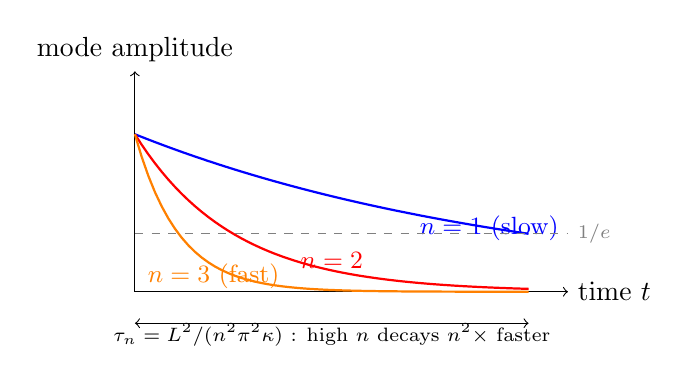
\begin{tikzpicture}[scale=1.0]
  \draw[->] (0,0) -- (5.5,0) node[right] {time $t$};
  \draw[->] (0,0) -- (0,2.8) node[above] {mode amplitude};

  % n=1 (slow decay)
  \draw[thick, blue, domain=0:5, samples=60]
    plot (\x, {2.0*exp(-\x*0.2)});
  \node[blue, font=\small] at (4.5, 0.8) {$n=1$ (slow)};

  % n=2 (medium decay)
  \draw[thick, red, domain=0:5, samples=60]
    plot (\x, {2.0*exp(-\x*0.8)});
  \node[red, font=\small] at (2.5, 0.4) {$n=2$};

  % n=3 (fast decay)
  \draw[thick, orange, domain=0:5, samples=60]
    plot (\x, {2.0*exp(-\x*1.8)});
  \node[orange, font=\small] at (1.0, 0.2) {$n=3$ (fast)};

  % Decay time annotation
  \draw[dashed, gray] (0, 0.74) -- (5.5, 0.74);
  \node[gray, font=\scriptsize, right] at (5.5, 0.74) {$1/e$};
  \draw[<->] (0,-0.4) -- (5.0/0.2*0.2,-0.4); % won't compile, simplified:
  \node[font=\scriptsize] at (2.5,-0.55)
    {$\tau_n = L^2/(n^2\pi^2\kappa)$ : high $n$ decays $n^2\times$ faster};
\end{tikzpicture}
\caption{Fourier mode amplitudes decay exponentially; high-order modes ($n \geq 2$) decay $n^2$ times faster than the fundamental mode. After a few decay times only $n=1$ remains, controlling the long-term approach to steady state.}
\end{figure}
}

\textbf{Fourier decomposition is the natural language of diffusion.} Because the diffusion operator is linear, sinusoidal modes are its eigenfunctions --- each mode evolves independently. This is the same spectral thinking used in gravity and magnetics to relate anomaly wavelength to source depth. In the thermal context, wavelength determines how quickly a mode decays.
}

\end{activity}